\documentclass{article}
\usepackage{fullpage}
\usepackage{mathtools}
\usepackage{hyperref}
\usepackage{amssymb}
\usepackage{graphicx}
\usepackage{placeins}
\usepackage{cancel}
\usepackage{verbatim}
\usepackage{floatrow}
\usepackage{caption}
\usepackage{ulem}

\newcommand\numberthis{\addtocounter{equation}{1}\tag{\theequation}}

\begin{document}

\title{Continuous Monte-Carlo Protein Folding}
\author{Bhareth Kachroo}
\date{\today}
\maketitle

\section{Introduction}
	Simulated protein folding is a minimization problem. A protein is such a complex, heterogeneous molecule that a direct simulation of Schrodinger or even Maxwell's equations is not currently feasible for realistic chain sizes (300 amino acids). Instead we assume thermal perturbation will eventually bring the protein to the deepest well in the energy landscape. If there were many minima of comparable sizes this would be useless, but evolution designs proteins that are robust to small changes in sequence, with a funneled energy landscape and guided folding process. As a result, real proteins fold much faster than we would expect for random thermal sampling \cite{fold}.

	The goal here is to capture some of the essential physics associated with this energy landscape using a simplified model, based on Giordani and Nakanishi's (GN) approach. \cite{GN} There are several factors influencing the landscape: the 20 types of amino acid interacting with each other, water molecules interacting with the amino acids, molecular chaperones and foldases that assist in folding. The GN model attempts to reproduce only the acid-acid interactions. This new model tries to improve on some of GN's deficiencies.

	The most commonly used first principles approach is Monte-Carlo simulation, which is also GN's approach. The most successful approach is actually homology modelling, using prior data on protein structure to look for patterns, but we're interested in the physics.
% end of section Introduction.

\section{Model}
	\subsection{GN Model}
		GN represent each amino acid as a point and the protein as a chain on a 2D grid, with the minimum distance equal to the bond length. The energy landscape is traverse by randomly moving an acid position to a nearest-neighbour such that the bond lengths remain fixed, approximating the strong energy associated with covalent bonds as opposed to other acid-acid interactions. The protein begins as a straight line, and follows the Metropolis algorithm. 

		The energy is calculated based on a randomized interaction between each type of acid at the start of the simulation. The interaction is only for adjacent acids that are not next to each other on the chain.

		This model has so many constraints it is unsuitable for a Monte Carlo simulation; it takes 25 steps to make the first move because only the endpoints can move at the beginning. This doesn't get much better: after 249 steps the result is only Fig. \ref{fig:gnfold}.

		\begin{figure}[h]
			\centering
			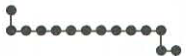
\includegraphics[width=0.2\textwidth]{GN_fold}
		    \caption{Folding after 249 time steps \cite{GN}}
			\label{fig:gnfold}
		\end{figure}
		
		This approach is extremely inefficient. It is also unstable, as shown by tests of the same protein folded repeatedly (with identical interactions) finding significantly different energy levels.
	% end of subsection GN Model.
	\subsection{Continuous Model}
	The model proposed here is mainly addressing the inefficiency of the GN model. Proteins are represented the same way, but in continuous 3D space. Varying the positions of the acids requires accounting for covalent bond energies and vibrations along the chain, so the variable to change is instead absolute angle in spherical coordinates. The bond length is preserved and now any angle can move, hugely reducing the number of wasted steps. If instead relative angle had been used, one section of the protein would rotate against the other, which would make progress in the later stages when the protein is mostly folded very slow. Instead one acid rotates and drags the rest of the protein over slightly, similar to the effect of pulling on coupled springs. See Figs.~\ref{fig:step2} and~\ref{fig:step3} for what this looks like.

	\begin{figure}[h]
	  \begin{floatrow}
	  \ffigbox{
	  \centering
	    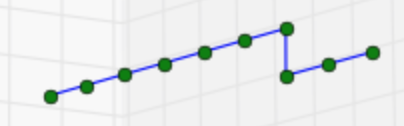
\includegraphics[width=0.3\textwidth]{step1}}
	    {\caption{Second Step}
	  \label{fig:step2}}
	  \ffigbox{
	  \centering
	    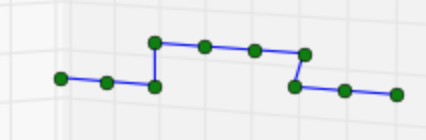
\includegraphics[width=0.3\textwidth]{step2}}
	  {\caption{Third Step}
	  \label{fig:step3}}
	  \end{floatrow}
	\end{figure}
	
	The energy calculation is also more realistic. Checking each unique acid pair for adjacency is~$O(n^2)$, so with the same asymptotic behaviour we can calculate each unique pair distance and use a radial potential to calculate the interaction energy. The potential used is two competing exponentials, as an approximation of the Lennard-Jones potential:

	\begin{equation}
		U(r) = 8 e^{-\frac{r}{0.2} } - e^{-\frac{r}{5} }
	\end{equation}

	\begin{figure}[h]
		\centering
		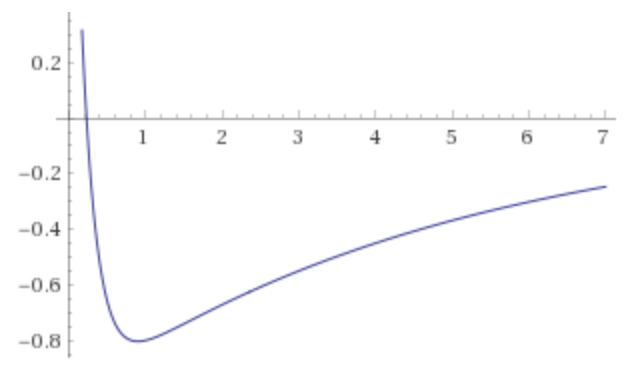
\includegraphics[width=0.5\textwidth]{expplot}
	    \caption{Plot of Potential}
		\label{fig:potential}
	\end{figure}
	
	The potential is shown in Fig.~\ref{fig:potential}. The idea is to encourage acids to be around the range of the bottom of the well, which is close to the bond length (one). This potential can be randomized to simulate different types of acids by changing the relative size of the coefficients and exponential parameters, but the repulse term should always have a larger coefficient and smaller exponential parameter. The effect would be to change the depth of the well, its position, or the intensity of the near-field repulsion.


	There is a restriction on how sharply the protein can bend at the joint of an amino acid, beyond what the potential provides, as the real amino acids are not located entirely at one point. This is approximated by restricting the relative angle between a triad of three adjacent acids to be greater than $\frac{\pi}{2} $ radians. 

% end of section Theory.

\section{Computational Method}
	Most of the new code is for geometry. Calculation of the potential requires absolute positions of the acids, called \texttt{positions()}. Since the first acid never moves, we start with that as the origin. Every successive absolute pair of angles is available. Transform the spherical coordinates with radius one to cartesian coordinates, and add these to the coordinates of the previous acid to get absolute coordinates for the next acid. 

	The restriction on relative angle is maintained by a mini-Monte-Carlo method: randomly shift the angles until one that isn't too acute is found (done by \texttt{try\_angles()}). This rarely takes more than three tries. The relative angle is calculated by using the central acid as the origin and finding the great circle distance between the two positions on the sphere, given latitude and longitude (by \texttt{relative\_angle()}). This gives angle:

	\begin{equation}
		A = \arccos (\sin \phi_1 \sin \phi_2 + \cos \phi_1 \cos \phi_2 \cos (\Delta \theta))
	\end{equation}

	where $\phi$ is the longitude and $\theta$ is the latitude. 

	The Metropolis algorithm (in \texttt{metropolis()}) picks a random index, calls \texttt{try\_angles()} to find a pair of new random angles, and recalculates the positions and total energy, using the Boltzmann factor for probability if the new energy is higher than the previous one.

	Accuracy is not well-defined, as we are not approximating a known mathematical structure, but trying to elucidate some properties of a physical process. The model is so simplified that the two cannot be directly compared beyond gross properties like stability.

	In a randomized simulation the error is typically just more randomness; here the major source of numerical error is the energy calculation, but the magnitude is still tiny even for realistic sized chains of n=300. This floating-point error only becomes significant for small magnitudes or an extremely large number of operations, neither of which apply. The end result of any error is simply something similar to operating with a slightly higher Boltzmann temperature.

	The most computationally demanding step is the energy calculation, which calculates distance and an energy exponential~$n^2/2$ times, where~$n$ is the number of amino acids. All other steps, like the $O(n)$ position calculation, are asympototically irrelevant. Then the time for a single Monte-Carlo step is~$O(n^2)$ and the total time is~$O(m n^2)$ where $m$ is the number of steps. The memory requirement is just~$O(n)$ to store the angles. Given the true protein-folding problem is NP-hard, those are pretty good efficiencies.

	\subsection{Testing}
		Direct tests are visual: are the acids too close together, do the angles change, are angles too acute. The method passes visual tests. Since the simulation is randomized, other tests are of component functions. The \texttt{metropolis()} function is straightforward and was tested in Lab 11, by checking the proportion of accepted moves vs. the energy difference. Relative angle is tested by trying it on some example angles and calculating by hand. Positions is tested by trying some simple starting angles and calculating the positions by hand. \texttt{try\_angles()} is tested by printing out the random angles it chooses and seeing which it returns, and whether it is in the appropriate range.
	% end of subsection Testing.

% end of section Computational Method.

\section{Results}
	\begin{figure}[h]
	  \begin{floatrow}
	  \ffigbox{
	  \centering
	    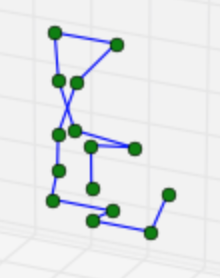
\includegraphics[width=0.2\textwidth]{step30}}
	    {\caption{Step 30}
	  \label{fig:step30}}
	  \ffigbox{
	  \centering
	    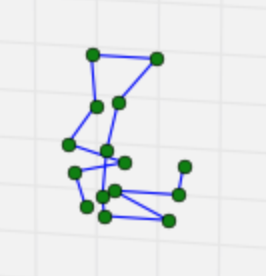
\includegraphics[width=0.2\textwidth]{step40}}
	  {\caption{Step 40}
	  \label{fig:step40}}
	  \end{floatrow}
	\end{figure}

	\begin{figure}[h]
	  \begin{floatrow}
	  \ffigbox{
	  \centering
	    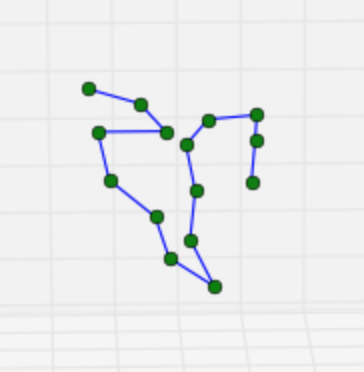
\includegraphics[width=0.2\textwidth]{step100}}
	    {\caption{Step 100}
	  \label{fig:step100}}
	  \ffigbox{
	  \centering
	    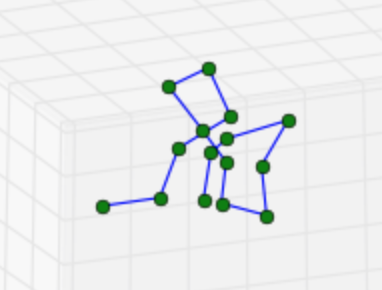
\includegraphics[width=0.2\textwidth]{step200}}
	  {\caption{Step 200}
	  \label{fig:step200}}
	  \end{floatrow}
	\end{figure}
	
	As seen in Figs. \ref{fig:step30} - \ref{fig:step200} the protein seems to become sufficiently complex by step 40 that after that it is impossible to distinguish which step it is by sight. Fig. \ref{fig:step30} and \ref{fig:step40} are from the same run, while the other two are both separate runs, as contrast.

	The energy varies with time as a scale-free power law, as seen in Figs. \ref{fig:e100} and \ref{fig:e200}. Compare this to Fig. \ref{fig:gncompare} and the difference is striking. The additional degrees of freedom clearly improve the speed of convergence, even at low T=1.

	\begin{figure}[h]
	  \begin{floatrow}
	  \ffigbox{
	  \centering
	    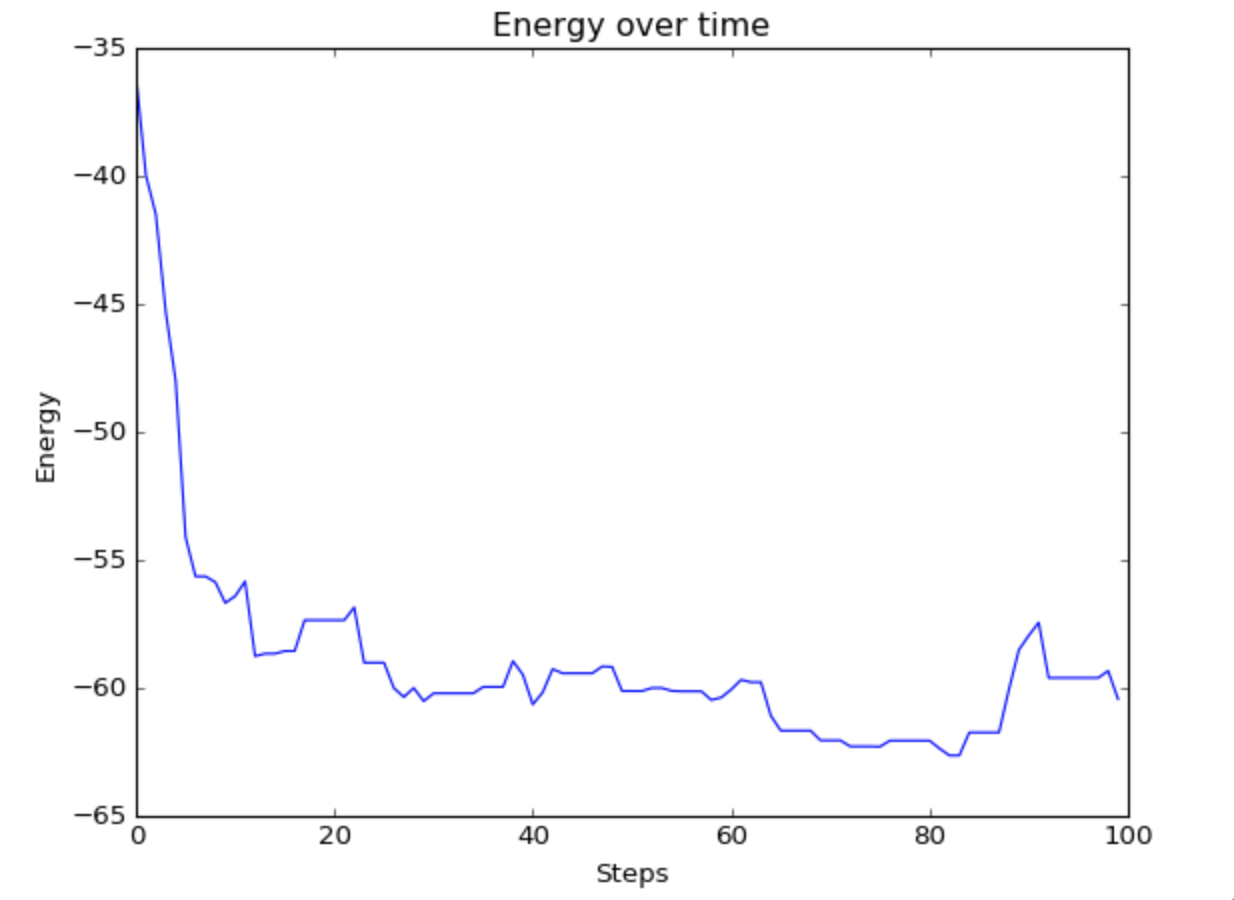
\includegraphics[width=0.5\textwidth]{e100}}
	    {\caption{Energy v. Time for 100 steps}
	  \label{fig:e100}}
	  \ffigbox{
	  \centering
	    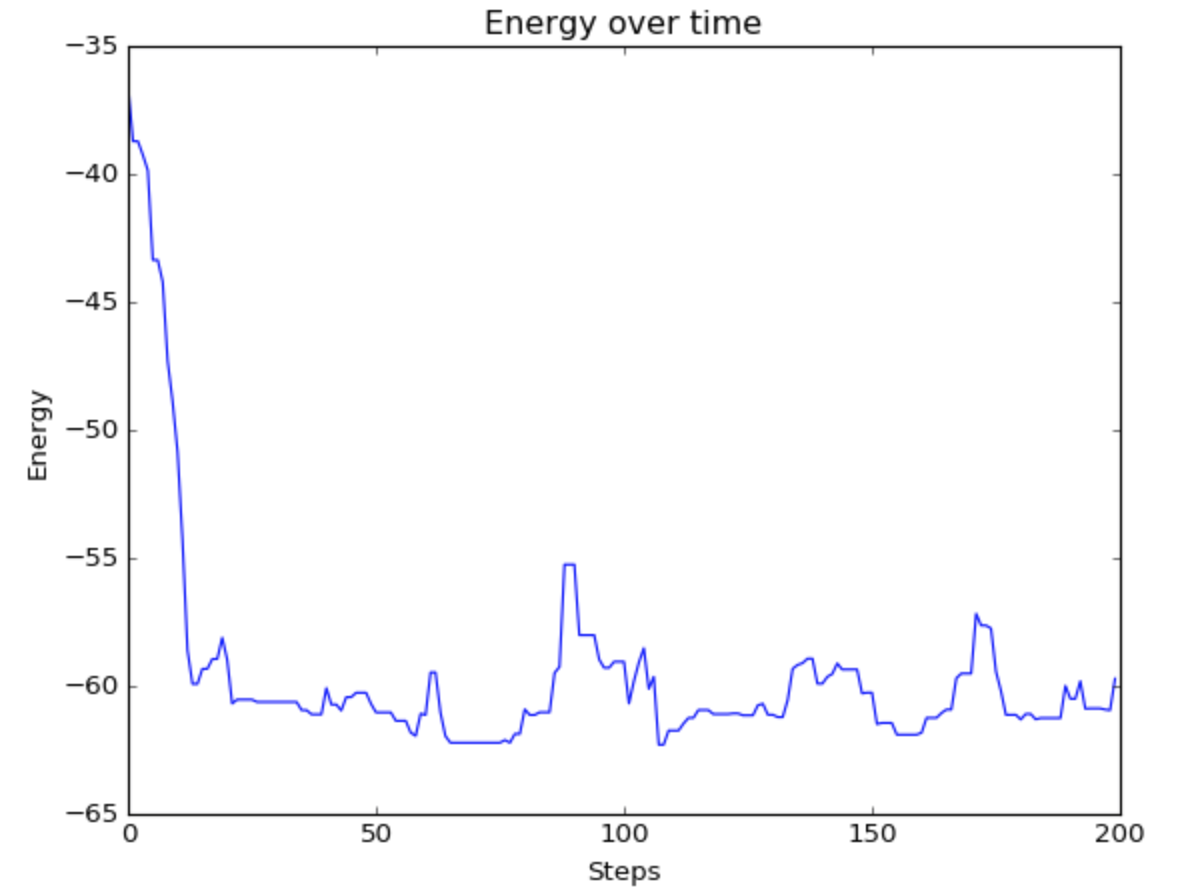
\includegraphics[width=0.5\textwidth]{e200}}
	  {\caption{Energy v. Time for 200 steps}
	  \label{fig:e200}}
	  \end{floatrow}
	\end{figure}

	\begin{figure}[h]
		\centering
		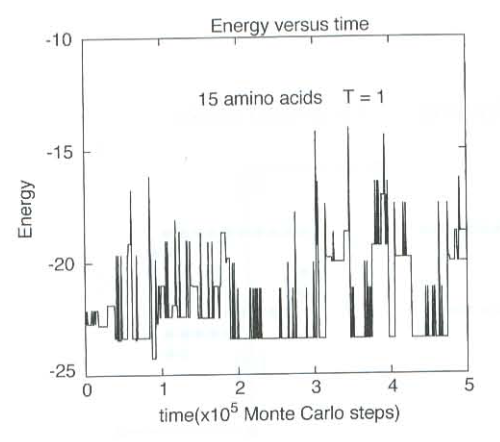
\includegraphics[width=0.5\textwidth]{compare}
	    \caption{GN's Energy vs. time \cite{GN}}
		\label{fig:gncompare}
	\end{figure}
	
	The algorithm is sensitive to temperature differences, as seen in Fig. \ref{fig:t7}, which is far more chaotic than T=1. In addition the higher temperatures result in a more strung-out chain as in Fig. \ref{fig:t10}.

	\begin{figure}[h]
	  \begin{floatrow}
	  \ffigbox{
	  \centering
	    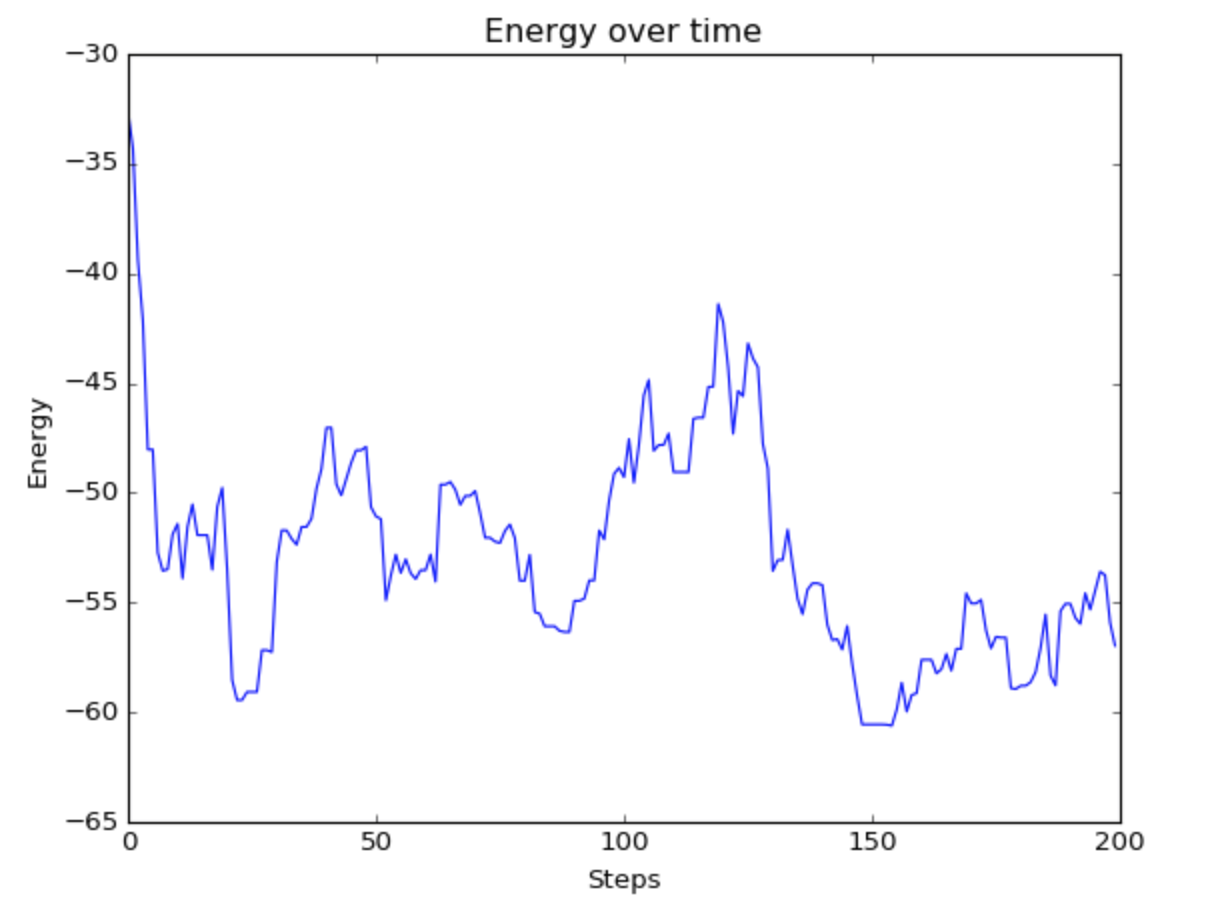
\includegraphics[width=0.5\textwidth]{t7}}
	    {\caption{Energy vs. Time for T=7}
	  \label{fig:t7}}
	  \ffigbox{
	  \centering
	    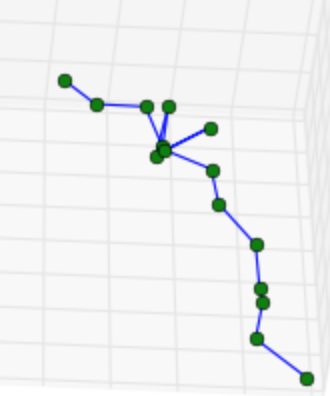
\includegraphics[width=0.5\textwidth]{t10ex}}
	  {\caption{Chain at step 100 for T=10}
	  \label{fig:t10}}
	  \end{floatrow}
	\end{figure}
	
	The behaviour of the best yet energy is fascinating, in Figs. \ref{fig:best500} and \ref{fig:best1000}. They also have scale-free power law curves, but the changes are sudden breakthroughs rather than steady improvements. The distance between breakthroughs also increases exponentially, and their size decreases. The total energy behaviour shows the system falling into deeper and deeper wells, and then climbing out. The early section shows funnel-like energy behaviour, with every run quickly falling toward a folded rather than extended structure. The energy range of minima after 50 steps is small enough (2, compared to a 33 difference between these states and unfolded) that these could be called substates at a general minimum.

	\begin{figure}[h]
	  \begin{floatrow}
	  \ffigbox{
	  \centering
	    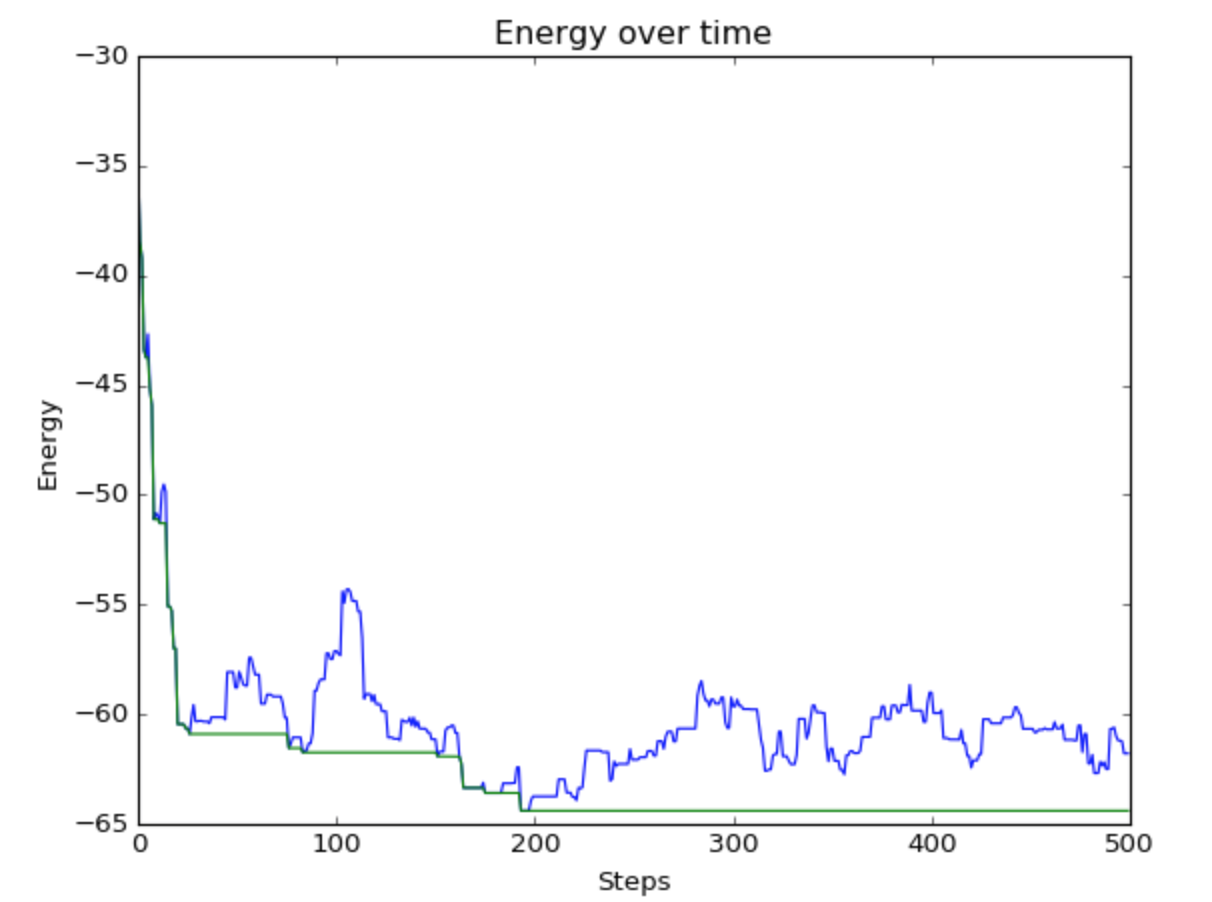
\includegraphics[width=0.5\textwidth]{beste500}}
	    {\caption{Best Energy v. Time}
	  \label{fig:best500}}
	  \ffigbox{
	  \centering
	    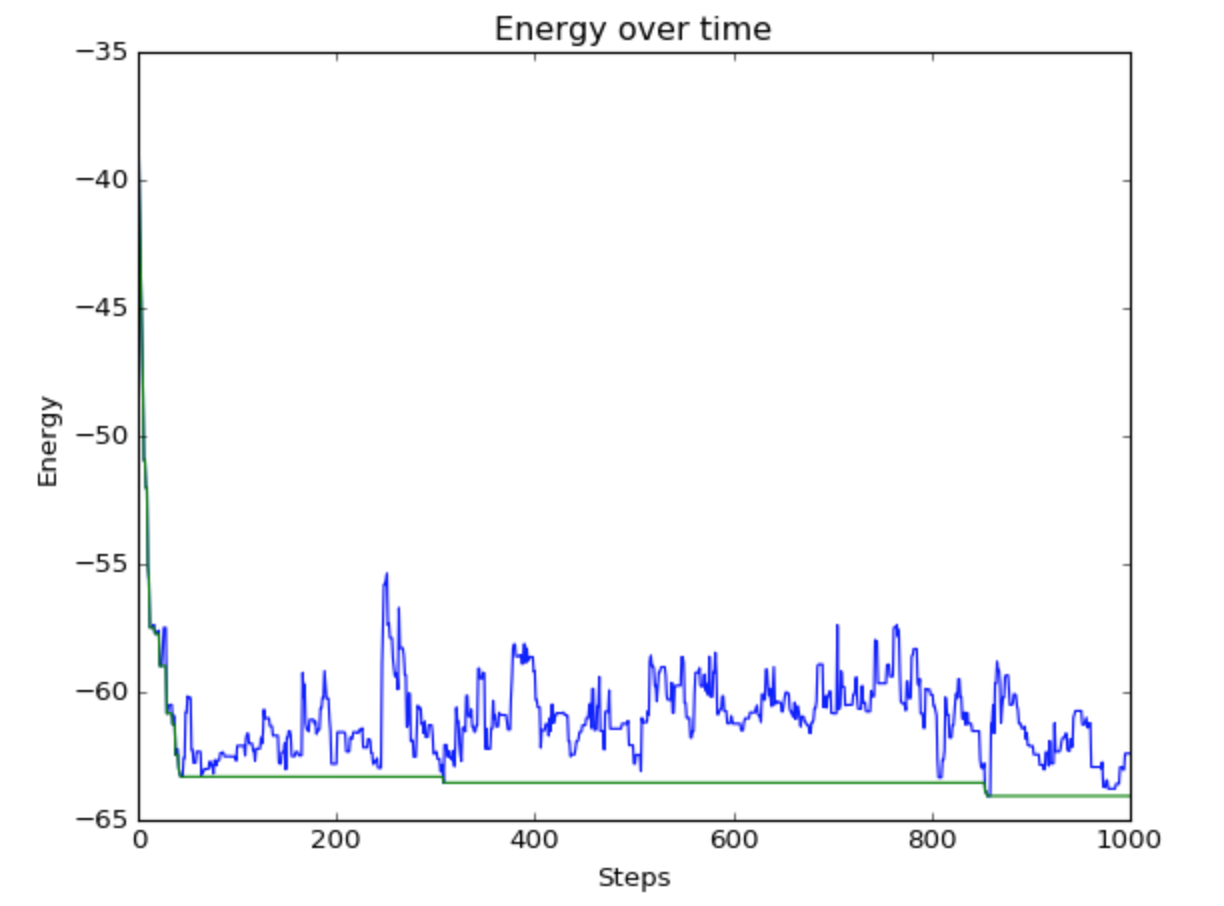
\includegraphics[width=0.5\textwidth]{beste1000}}
	  {\caption{Best Energy v. Time}
	  \label{fig:best1000}}
	  \end{floatrow}
	\end{figure}
	

	The very long-range behaviour shows a stabilization over time. The limit for this energy function at a constant temperature seems to be around -65. As in Figs. \ref{fig:step5000}, \ref{fig:t5} the higher temperatures stabilize around a higher average energy, with a larger deviation. The density of the wells appears to stabilize as well, suggesting a periodic aspect to the modulation, which deserves spectral analysis.

	\begin{figure}[h]
	  \begin{floatrow}
	  \ffigbox{
	  \centering
	    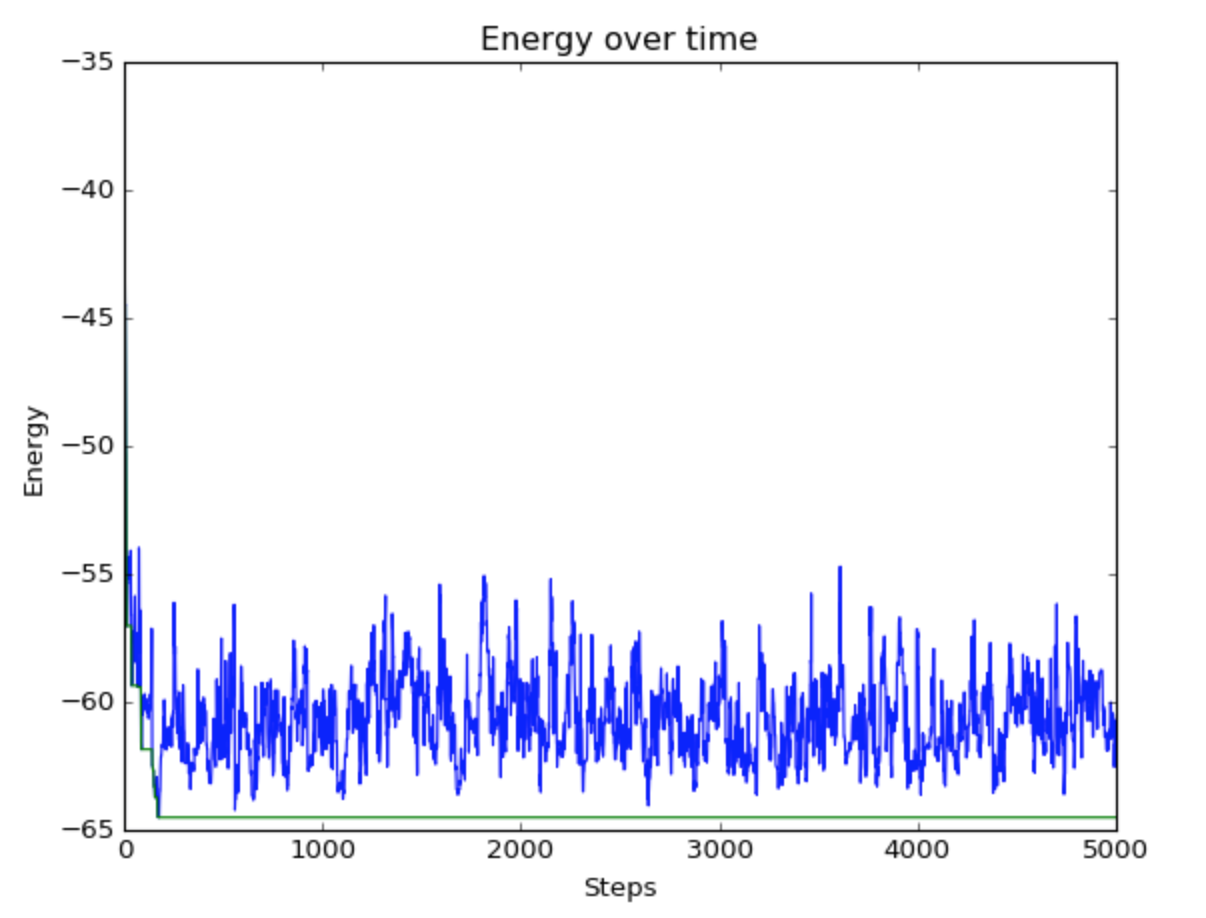
\includegraphics[width=0.5\textwidth]{step5000}}
	    {\caption{Long-range Stabilization T=1}
	  \label{fig:step5000}}
	  \ffigbox{
	  \centering
	    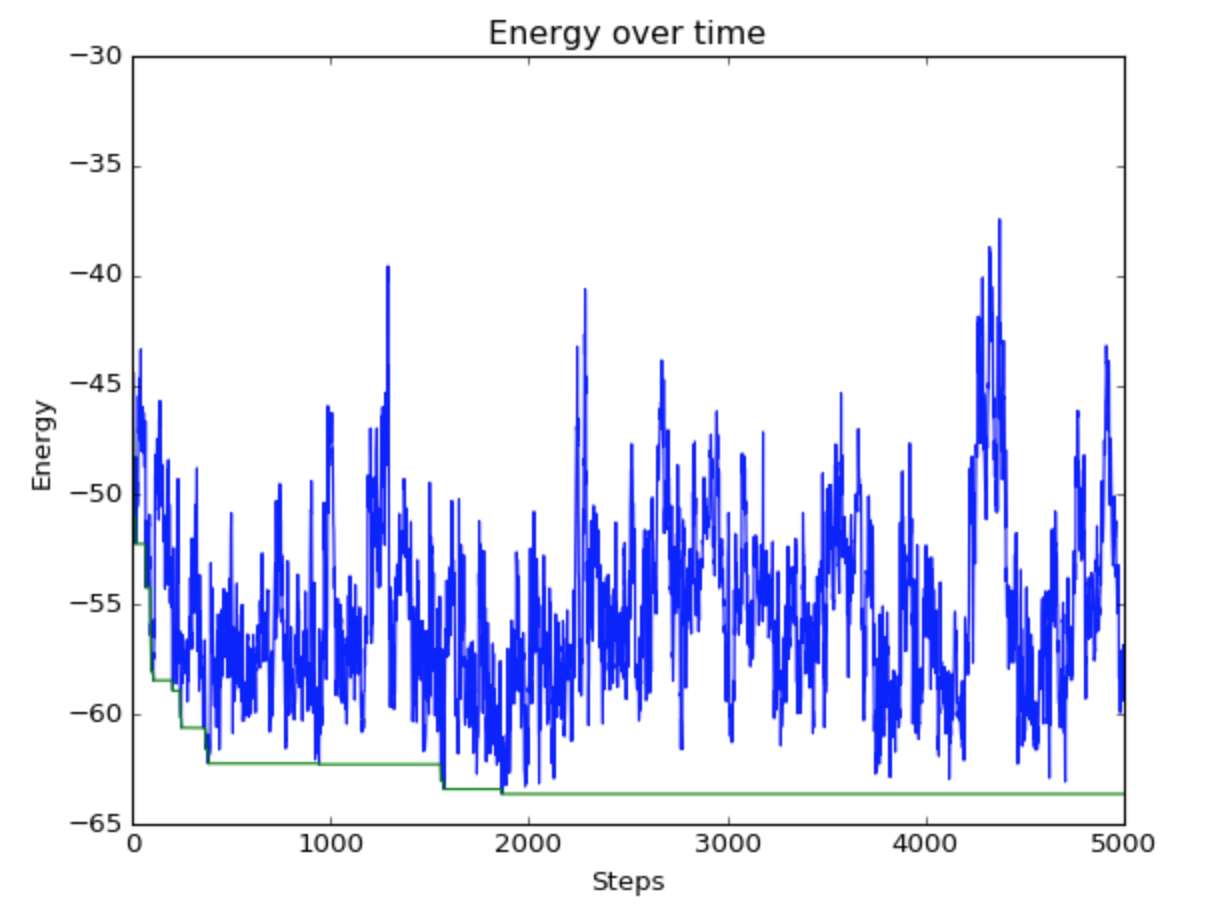
\includegraphics[width=0.5\textwidth]{longt5}}
	  {\caption{Long-range T=5}
	  \label{fig:t5}}
	  \end{floatrow}
	\end{figure}
	
	There is also improved stability for repeated runs as compared to the GN model in Fig. \ref{fig:gnstab}. Fig. \ref{fig:stab} shows energies never quite settling down, but clearly occupying the same range, as opposed to different levels in Fig. \ref{fig:gnstab}.

	\begin{figure}[h]
	  \begin{floatrow}
	  \ffigbox{
	  \centering
	    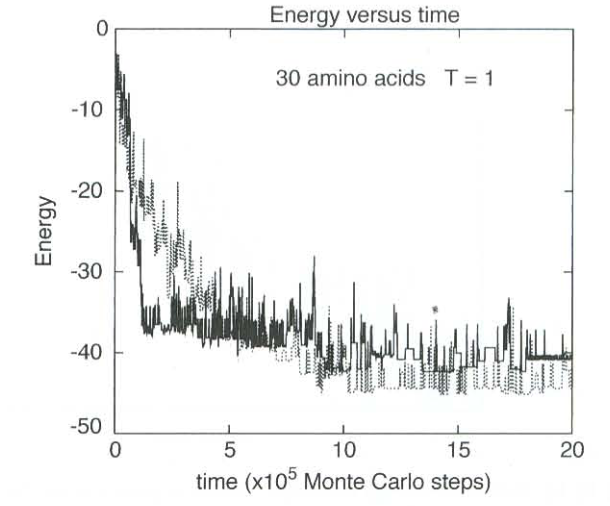
\includegraphics[width=0.5\textwidth]{gb_stab}}
	    {\caption{Stability for GN Model \cite{GN}}
	  \label{fig:gnstab}}
	  \ffigbox{
	  \centering
	    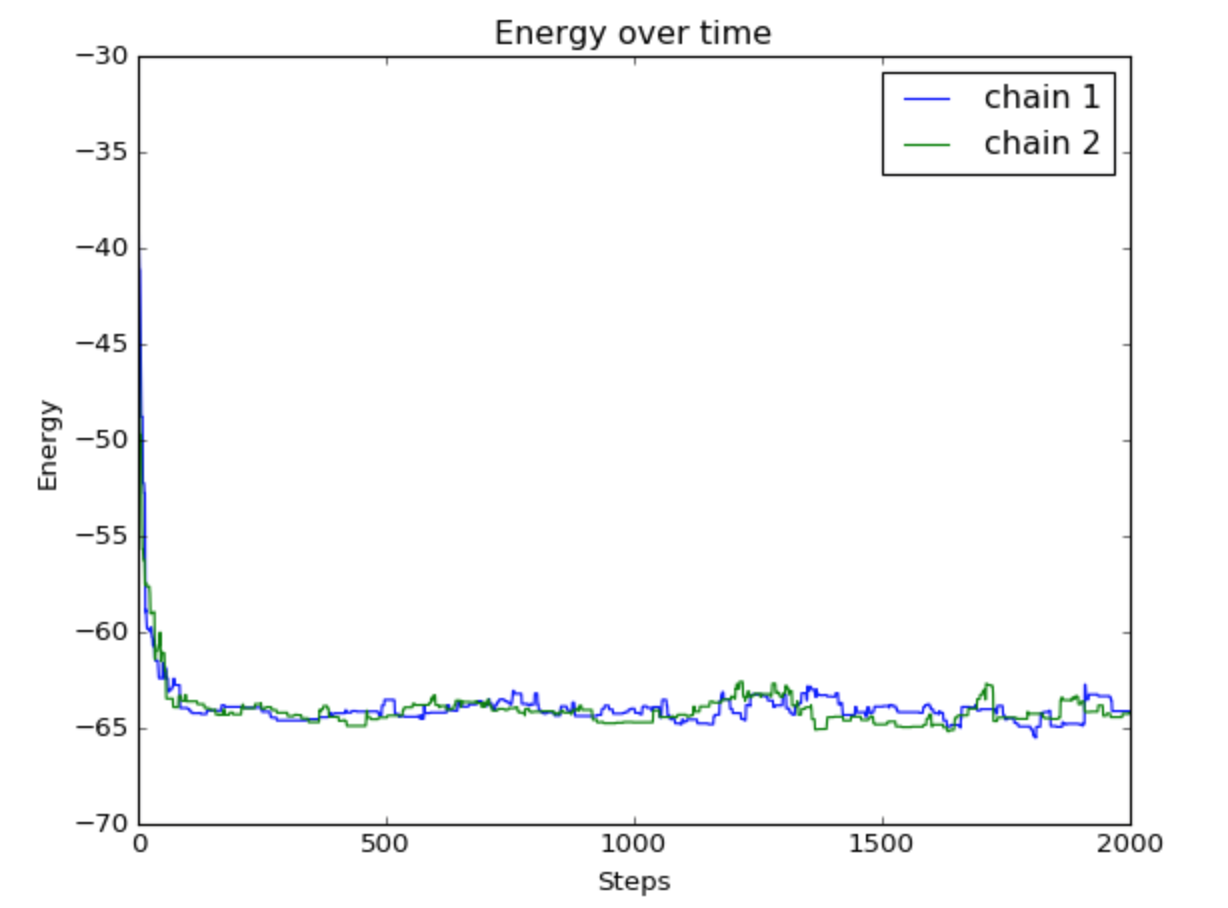
\includegraphics[width=0.5\textwidth]{stability}}
	  {\caption{Stability for Repeated Runs at T=0.2}
	  \label{fig:stab}}
	  \end{floatrow}
	\end{figure}

	Figs. \ref{fig:x1} to \ref{fig:y2} shows the two structures at step 5000 from Fig. \ref{fig:stab}. While they are not identical, they have clear structural similarities as compared to the other figures of protein structures above. The structural stability of the algorithm and energy landscape suggest this approach is accurate in capturing the general properties of real protein folding.

	\begin{figure}[h]
	   \begin{floatrow}
	   \ffigbox{
	   \centering
	     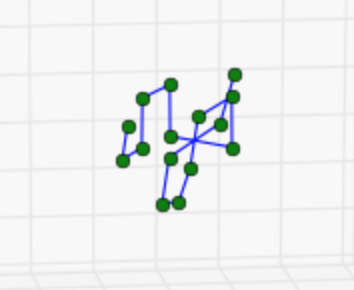
\includegraphics[width=0.3\textwidth]{x1}}
	     {\caption{First Chain View 1}
	   \label{fig:x1}}
	   \ffigbox{
	   \centering
	     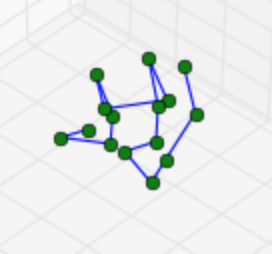
\includegraphics[width=0.3\textwidth]{y1}}
	   {\caption{First Chain View 2}
	   \label{fig:y1}}
	   \end{floatrow}
	 \end{figure}

	 \begin{figure}[h]
	   \begin{floatrow}
	   \ffigbox{
	   \centering
	     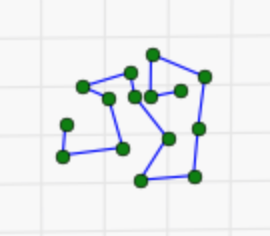
\includegraphics[width=0.3\textwidth]{x2}}
	     {\caption{Second Chain View 1}
	   \label{fig:x2}}
	   \ffigbox{
	   \centering
	     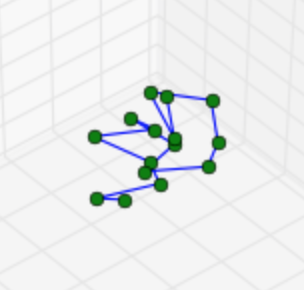
\includegraphics[width=0.3\textwidth]{y2}}
	   {\caption{Second Chain View 2}
	   \label{fig:y2}}
	   \end{floatrow}
	 \end{figure}
	
% end of section Results.

\section{Conclusion}
	The approach discussed here is a much better representation of protein folding than the original GN model, displaying funneling and structural stability on repetition. While the energy calculation is more complicated, sensible degrees of freedom reduce the number of Monte-Carlo steps required (from $20*10^5$ to $100$) so greatly that it runs much faster.

	Next steps would be randomizing the potential energy variables, examining the effects of simulated annealing, and seeing if any typical secondary protein structures can be reproduced like alpha helices.

% end of section Conclusion.

\begin{thebibliography}{9}

  \bibitem{GN}
  Giordano, N. and Nakanishi, H. (2006). \textit{Computational physics}. New Delhi: Dorling Kindersley.

  \bibitem{fold}
  Chen, M., Lin, X., Zheng, W., Onuchic, J. and Wolynes, P. (2016). \textit{Protein Folding and Structure Prediction from the Ground Up: The Atomistic Associative Memory, Water Mediated, Structure and Energy Model}. The Journal of Physical Chemistry B, 120(33), pp.8557-8565.
\end{thebibliography}

\end{document}